\graphicspath{{./sozai/}}
\chapter{問題定義}\label{definition}

シミュレーション作業は各階層ごとに行う.
各階は4つのホールドと呼ばれる一定の広さで区切られたスペースが存在し, 各ホールドに詰め込む車の情報は決まっている.
本稿では複数種類のある階層の中で, 4つのホールドを持つ単純な階層のデータを用いて行う.


\section{用語定義}
本研究で扱う船の航海等に関する専門用語の定義をする\cite{takeda}.

\begin{itemize}
    \item 席割 \\
    注文一つ一つを船のホールドに割り当てる作業.

    \item シミュレーション \\
    席割で決まった自動車を一台ずつホールド内の領域に貼り付ける作業.

    \item  プランナー \\
    席割やシミュレーションを考える作業者.

    \item  オペレーター\\
    港で自動車をホールドまで運転して積み降ろしをする作業者.

    \item デッキ \\
    船の内部の階層.

    \item ホールド \\
    各デッキ内を一定間隔の領域で仕切られた空間.
    本研究では, 各デッキは4つのホールドを持つ.

    \item セグメント \\
    隣接するいくつかのホールドをまとめた空間.
    本研究では, ホールド1,2とホールド3,4をまとめたものをそれぞれセグメント1, セグメント2と呼ぶ.

    \item ランプ \\
    上下のデッキに移動するために各デッキの特定ホールドについているスロープ.

    \item 積み地 \\
    注文における自動車を積む港.

    \item 揚げ地 \\
    注文における自動車を降ろす港.

\end{itemize}


\section{入力情報}
本研究で扱う2種類の情報について述べる.

\begin{itemize}
    \item 車体情報 \\
    車の数, 種類, 大きさ, 積み地, 揚げ地, 指定のホールド. \\
    本研究では実際のプランで使われているデータを利用した.
    \item 船体情報 \\
    船体の大きさ, 各階のランプの位置, 船内の障害物の位置や大きさ. \\
    本研究では実際の図面データを元に手入力で行った.

\end{itemize}
入力情報のうち車体情報の例を表\ref{table21}に示し, 船内図を図\ref{figure21}に示す.

\begin{table}[htbp]
    \tabcolsep = 10pt
    % \renewcommand{\arraystretch}{0.7}
    \caption{車体情報の例}
    \label{table21}
    \begin{center}
    \begin{tabular}{rcccrcrr} \hline
    番号 & 車種 & 積み地 & 揚げ地 & 数量 & ホールド & 横幅 & 高さ \\ \hline
    1 & Prius & A港 & E港 & 100 & 1 & 200 & 500 \\
    2 & Prius & A港 & E港 & 100 & 2 & 200 & 500 \\
    3 & Aqua & B港 & F港 & 30 & 2 & 250 & 450 \\
    4 & Carolla & C港 & G港 & 60 & 3 & 180 & 480 \\
    5 & Lexus & C港 & G港 & 40 & 3 & 230 & 510 \\
    6 & Lexus & D港 & H港 & 100 & 4 & 230 & 420 \\
    \hline
    \end{tabular}
    \end{center}
    \end{table}

\begin{figure}[htbp]
    \centering
    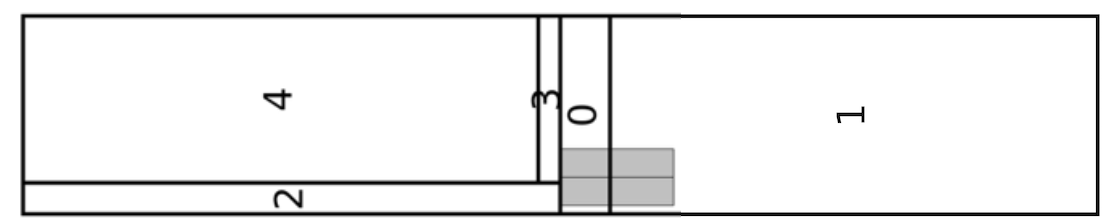
\includegraphics[scale=0.5, bb=0 0 30 30]{2-sennaizu.png}
    \caption{船内図の例(仮)}
    \label{figure21}
\end{figure}

\section{出力}
詰め込むことのできなかった車の台数と配置図を出力する. \\
配置図の例を図\ref{figure22}に示す.\\


\begin{figure}[H]
    \centering
    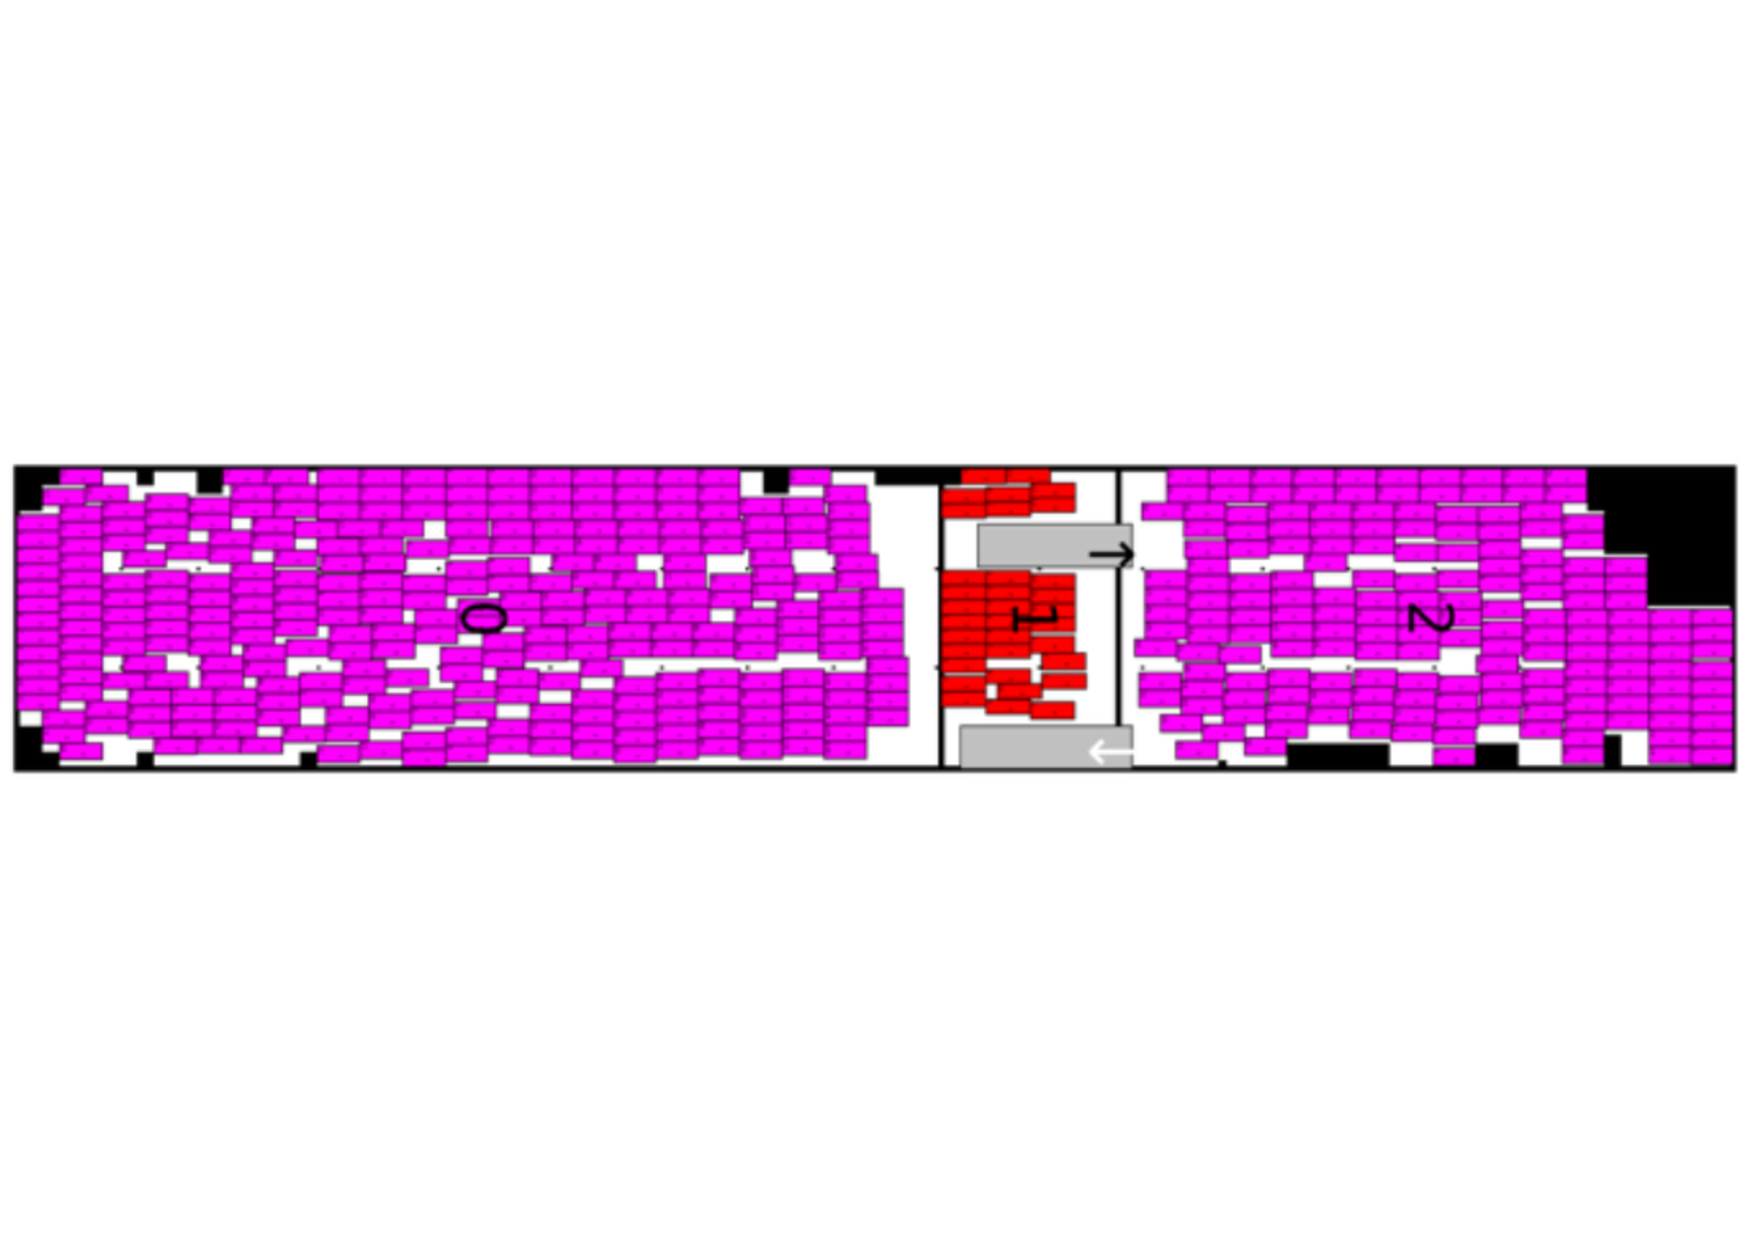
\includegraphics[scale=0.5, bb = 0 0 1 10]{2ship.pdf}
    \caption{車両配置図の例(仮)}
    \label{figure22}
\end{figure}


% \begin{table}[htbp]
%     \tabcolsep = 15pt
%     \renewcommand{\arraystretch}{0.8}
%     \caption{出力の例1}
%     \label{table22}
%     \begin{center}
%     \begin{tabular}{rcccrrrr} \hline
%     番号 & 車種 & 積み地 & 揚げ地 & 数量 & ホールド & 横幅 & 高さ \\ \hline
%     1 & Prius & A港 & E港 & 3 & 1 & 200 & 500 \\
%     2 & Prius & A港 & E港 & 5 & 2 & 200 & 500 \\
%     3 & Aqua & B港 & F港 & 10 & 4 & 250 & 450 \\
%     \hline
%     \end{tabular}
%     \end{center}
%     \end{table}
